% !TEX root = ../thesis.tex
\chaptermark{Návrh}
\phantomsection
\addcontentsline{toc}{chapter}{Návrh}
\chapter{Návrh používateľského rozhrania}

\label{summary}

Používateľské rozhranie bolo centrované okolo ideálneho používateľa pomocou viacerých iterácií. Dve hlavné iterácie boli vykonané používateľskými testami. Pri formálnom spôsobe sme použili interview a dotazník s otázkami ohľadne použiteľnosti a konzistencii. Primárne bol používaný prototypovací nástroj Figma \footnote{https://www.figma.com/} pri všetkých prototypoch.



\section{Konceptuálny model}

	Ako môžeme vidieť na obrázku \ref{scenar} na začiatku sú informácie o používateľovi, technické zručnosti a Bio. Následne vidíme scenár primárnej úlohy modelu začiatku sú informácie o používateľovi, technické zručnosti a Bio. Následne vidíme scenár primárnej úlohy modelu

Používateľské rozhranie bolo vytvárané postupne s pomocou cvičení z predmetu UX. Vybranie správneho smeru bolo zložité, nakoľko bolo viacero časti bakalárskej práce, ktoré bolo možné implementovať do používateľského prostredia. Ako prvú časť bolo potrebné vybrať personu, ktorá má predstavovať ideálneho zákazníka/používateľa a to bol majiteľ esportového tímu. Následne sme jej vytvorili scenár, ktorý bol potrebný na vytvorenie prvého prototypu. 

\begin{figure}[h!]
	
	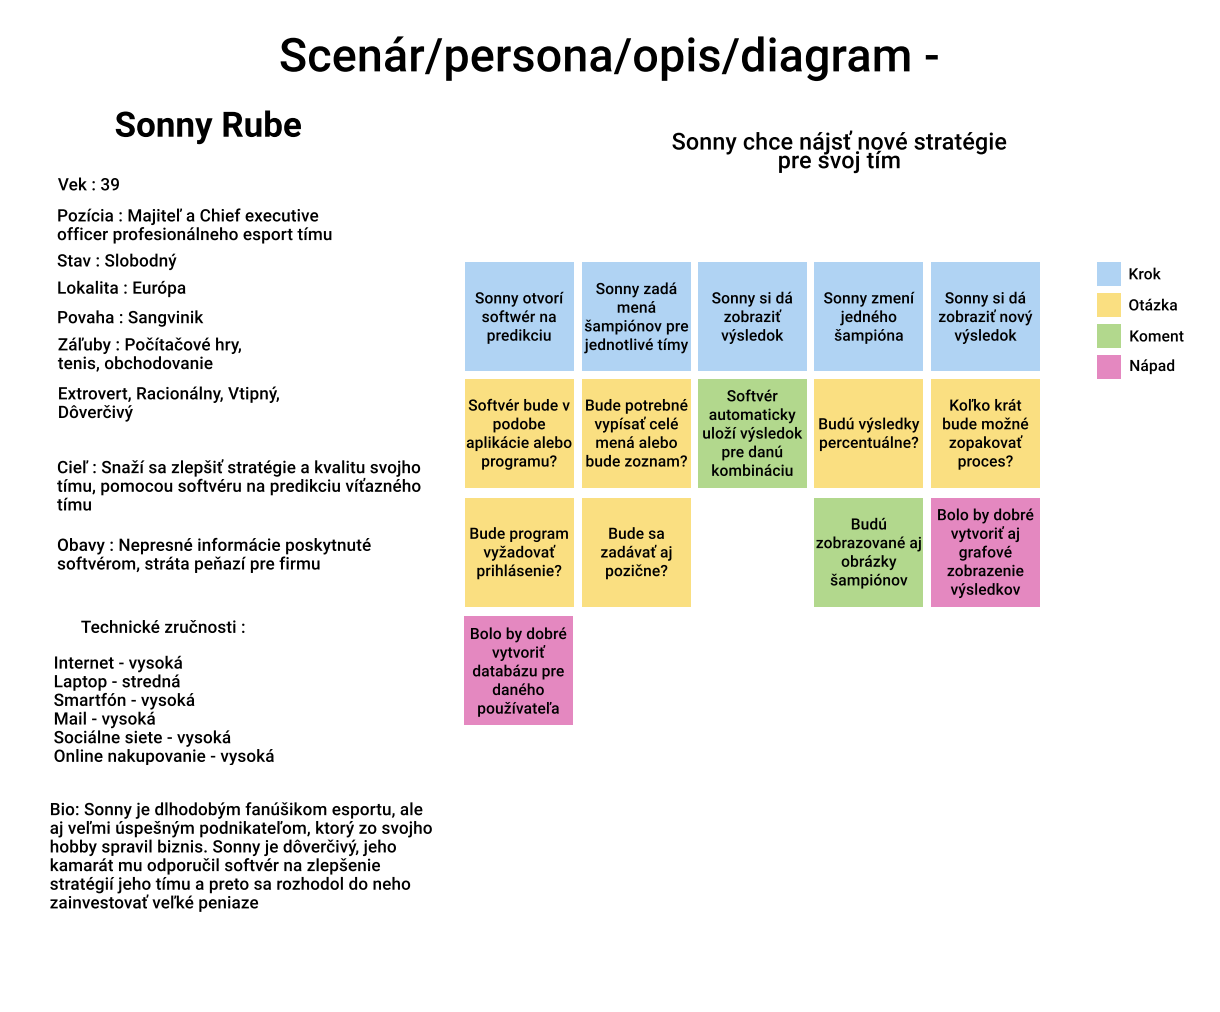
\includegraphics[width=.9\textwidth]{figures/scenar}
	
	\centering
	
	\caption{ Informácie o používateľovi \label{scenar}}
	
\end{figure}

\section{Návrh postupností obrazoviek}

Návrh postupností obrazoviek máme rozdelený na 5 častí, podľa nás najdôležitejších častí, ktoré sú nevyhnutné na správny chod, konkrétne obrazovky sú na obrázku \ref{jednanula}. V nasledujúcich častiach si ich predstavíme.
\subsubsection{Prihlasovanie}

Na prvej obrazovke sa nachádza prihlasovanie do účtu s možnosťou zabudnutého hesla.

\subsubsection{Prázdna obrazovka}

Následné je presunutie na prázdnu obrazovku, kde je potrebné vyplniť miesta na vypočítanie pravdepodobnosti daného tímu na výhru.

\subsubsection{Vyplnená obrazovka}

Potrebujeme vyplniť všetky prázdne políčka šampiónmi z hry League of Legends.

\subsubsection{Výsledková obrazovka}

Po vyplnení môžeme stlačiť tlačidlo vypočítať, ktoré v praxi zoberie zadané tímy a pošle ich umelej inteligencii, ktorá vypočíta percentuálnu výhru obidvoch tímov. Výsledky z tohto pokusu môžeme uložiť.

\subsubsection{História}

To nás automaticky prenesie na ďalšiu obrazovku histórie. V histórii si môžeme prezrieť predošlé vykonané pokusy a ich podrobnosti. Z histórie možeme následne rovno prejsť na nový prípad.

\begin{figure}[h!]
	
	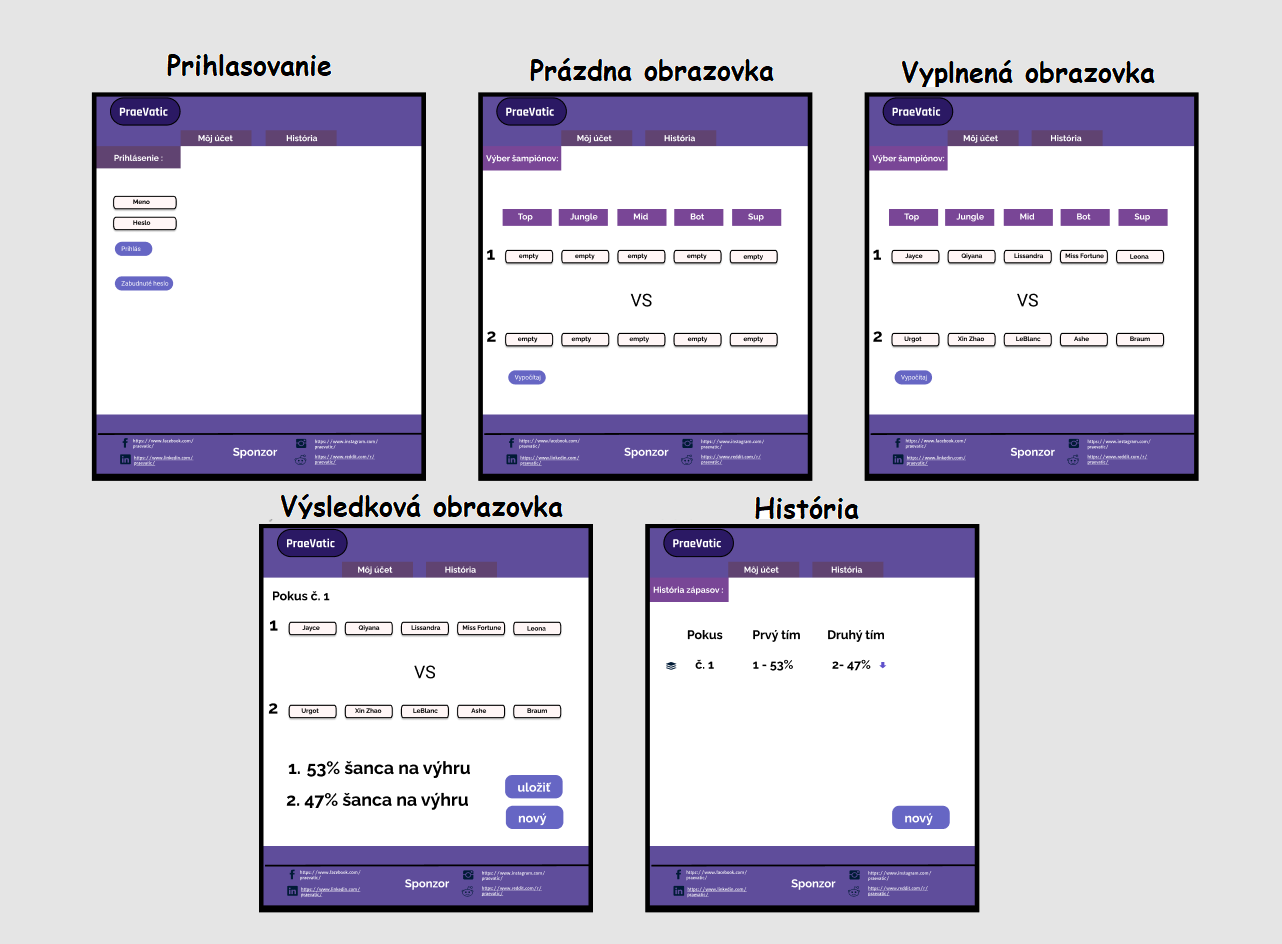
\includegraphics[width=.9\textwidth]{figures/postupnost}
	
	\centering
	
	\caption{ Postupnosť obrazoviek prototypu z nástroja figma \label{jednanula}}
	
\end{figure}

\section{Prvý prototyp}

Aktuálny prototyp v nástroji figma\footnote{https://www.figma.com/proto/ze1H0AqlBQMaAQzBSOqKDf/UX-odovzdavky?node-id=2\%3A2\&starting-point-node-id=2\%3A2\&scaling=min-zoom}, si môžete prezerať.  
Takisto bolo natočené video \footnote{https://www.youtube.com/watch?v=2UFsyUZgpUM\&t=11s} s ukážkou vykonanie scenárov.
\\ \\
Pri prvom prototype sme použili všetky informácie, ktoré sme objasnili pri prvých bodoch ako scenár. Hlavná bola použiteľnosť a jednoduchosť použitia softvéru na predikciu. Kolorizácia je okolo fialovej farby typ monochromatic. Používateľské testy boli až po vytvorení prvého prototypu. 


\begin{figure}[h!]
	
	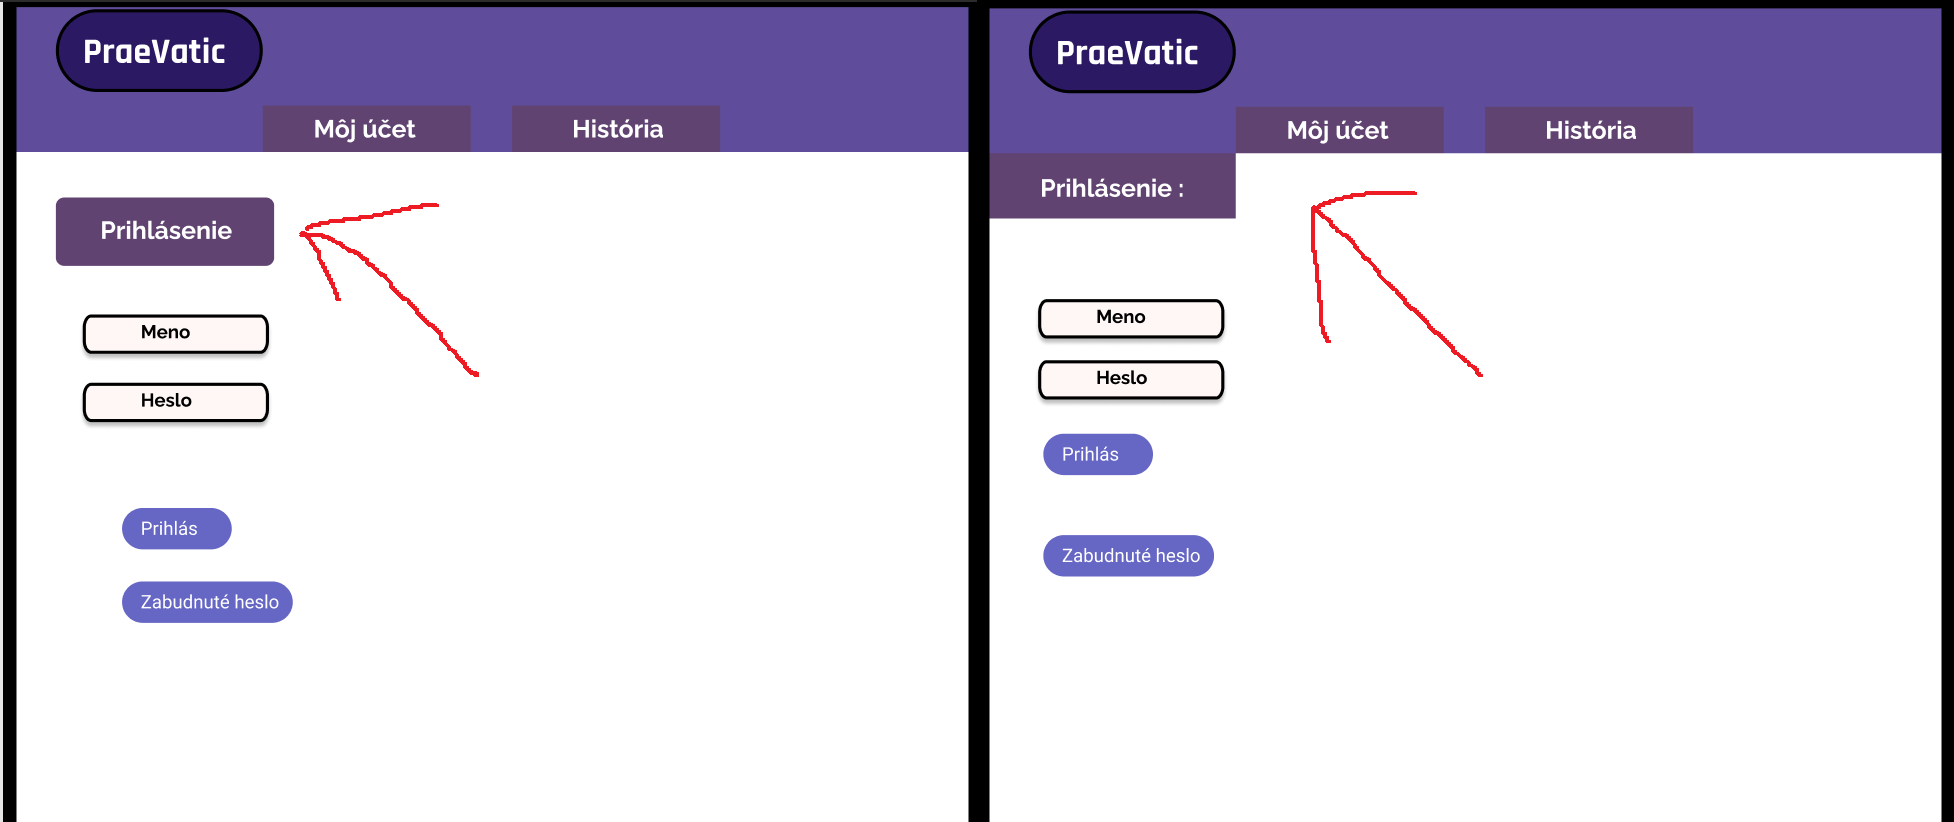
\includegraphics[width=.9\textwidth]{figures/predtym}
	
	\centering
	
	\caption{ Ukážka prvej zmeny v prototype na prihlásenie\label{predtym}}

	
	
\end{figure}


Testeri sa pri pokyne prihlásiť sa pokúšali stlačiť fialový nadpis Prihlásenie, to ale nebolo možné a pravdepodobne to bolo mätúce. Preto sme sa rozhodli ho pripojiť k hornej časti a zmeniť oblé okraje. Zmenu je vidno na obrázku : \ref{predtym}


\begin{figure}[h!]
	
	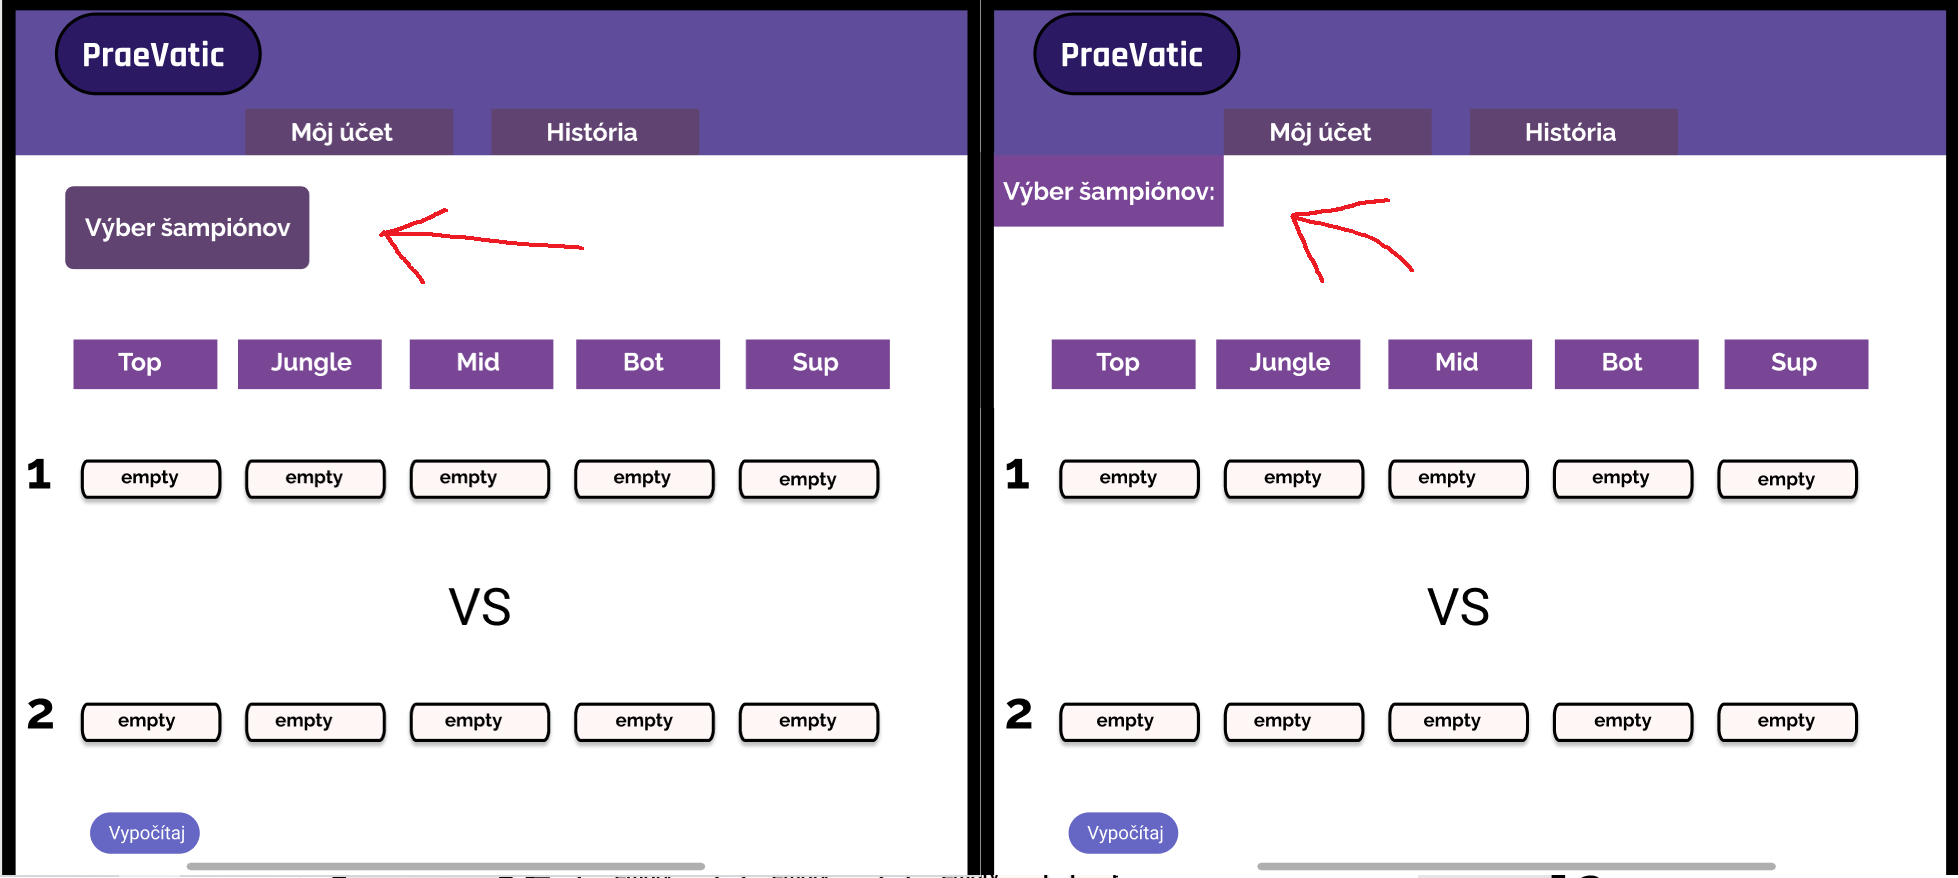
\includegraphics[width=.9\textwidth]{figures/2}
	
	\centering
	
	\caption{Ukážka zmeny v prototype na výber šampiónov\label{2}}
	
\end{figure}

	Podobne ako pri prvej zmene sa testeri pokúšali vybrať šampiónov pomocou nadpisu Výber šampiónov, tak sme ho presunuli k okraju, zmenili farbu a zrušili oblé okraje, ako môžeme vidieť na obrázku : \ref{2} 

\begin{figure}[h!]
	
	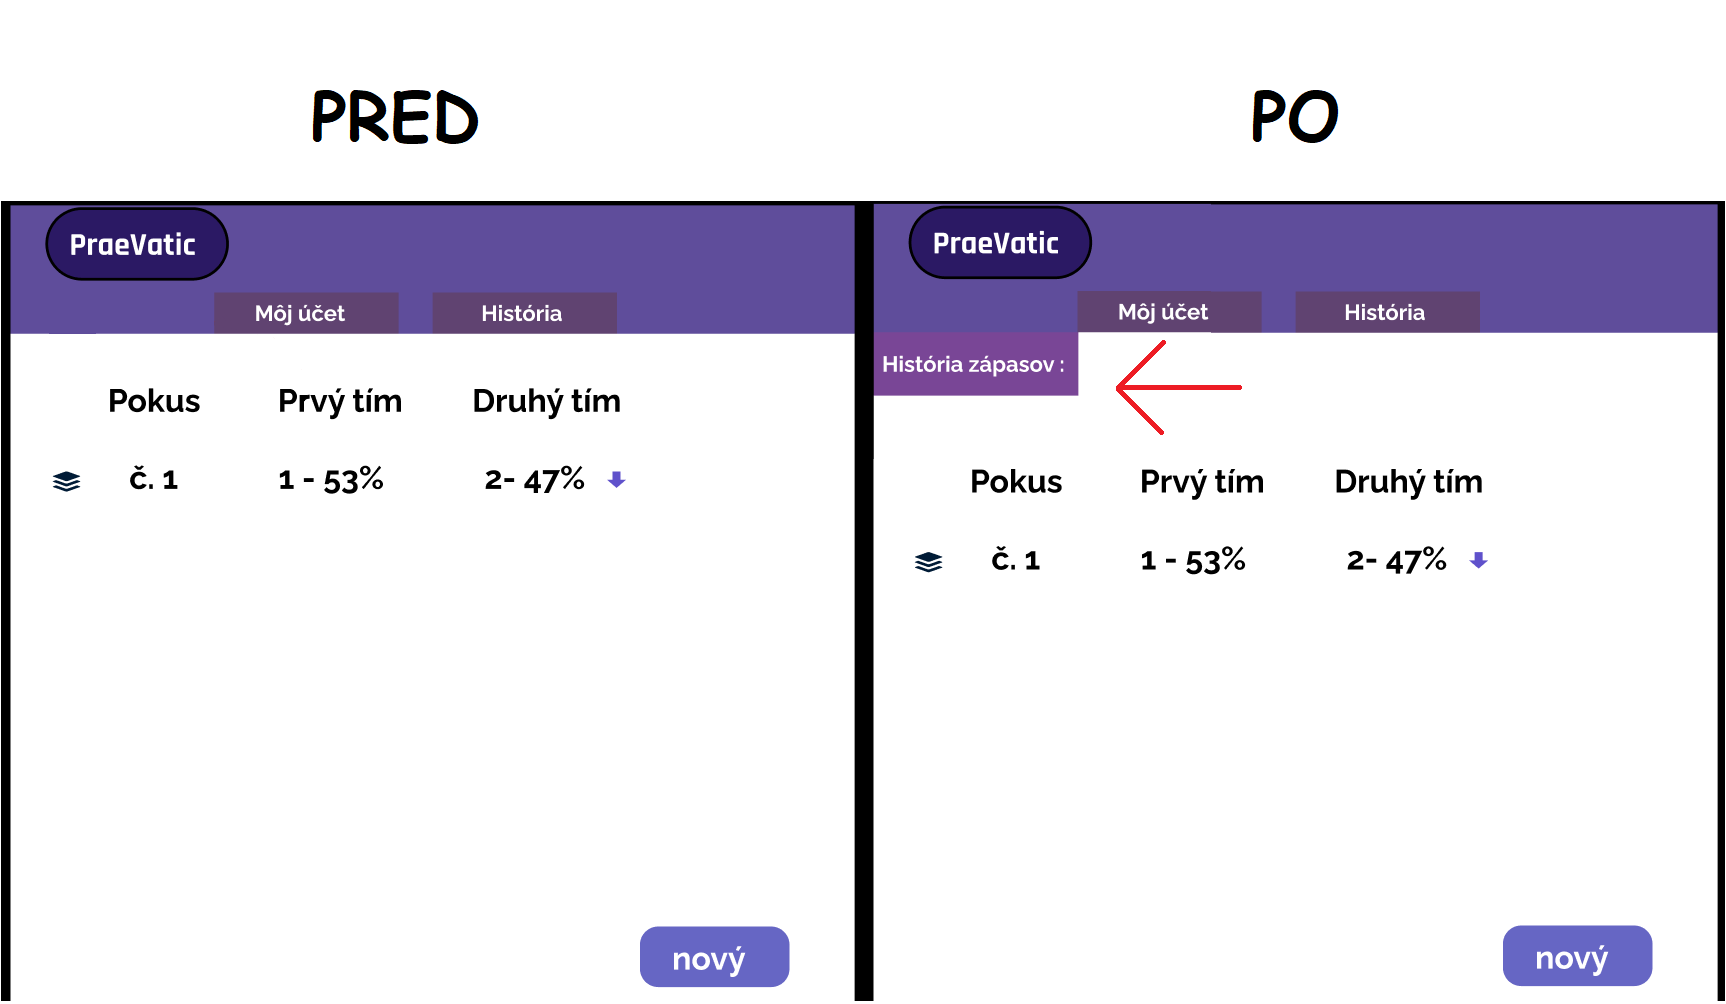
\includegraphics[width=.9\textwidth]{figures/3}
	
	\centering
	
	\caption{ Ukážka zmeny pri histórii zápasov \label{3}}
	
\end{figure}

Na stránke histórie nebolo testerom hneď jasné o čo sa jedná, tak sme sa rozhodli pridať popis História zápasov na objasnenie, ako vidíme na obrázku \ref{3}.
\\



\begin{figure}[h!]
	
	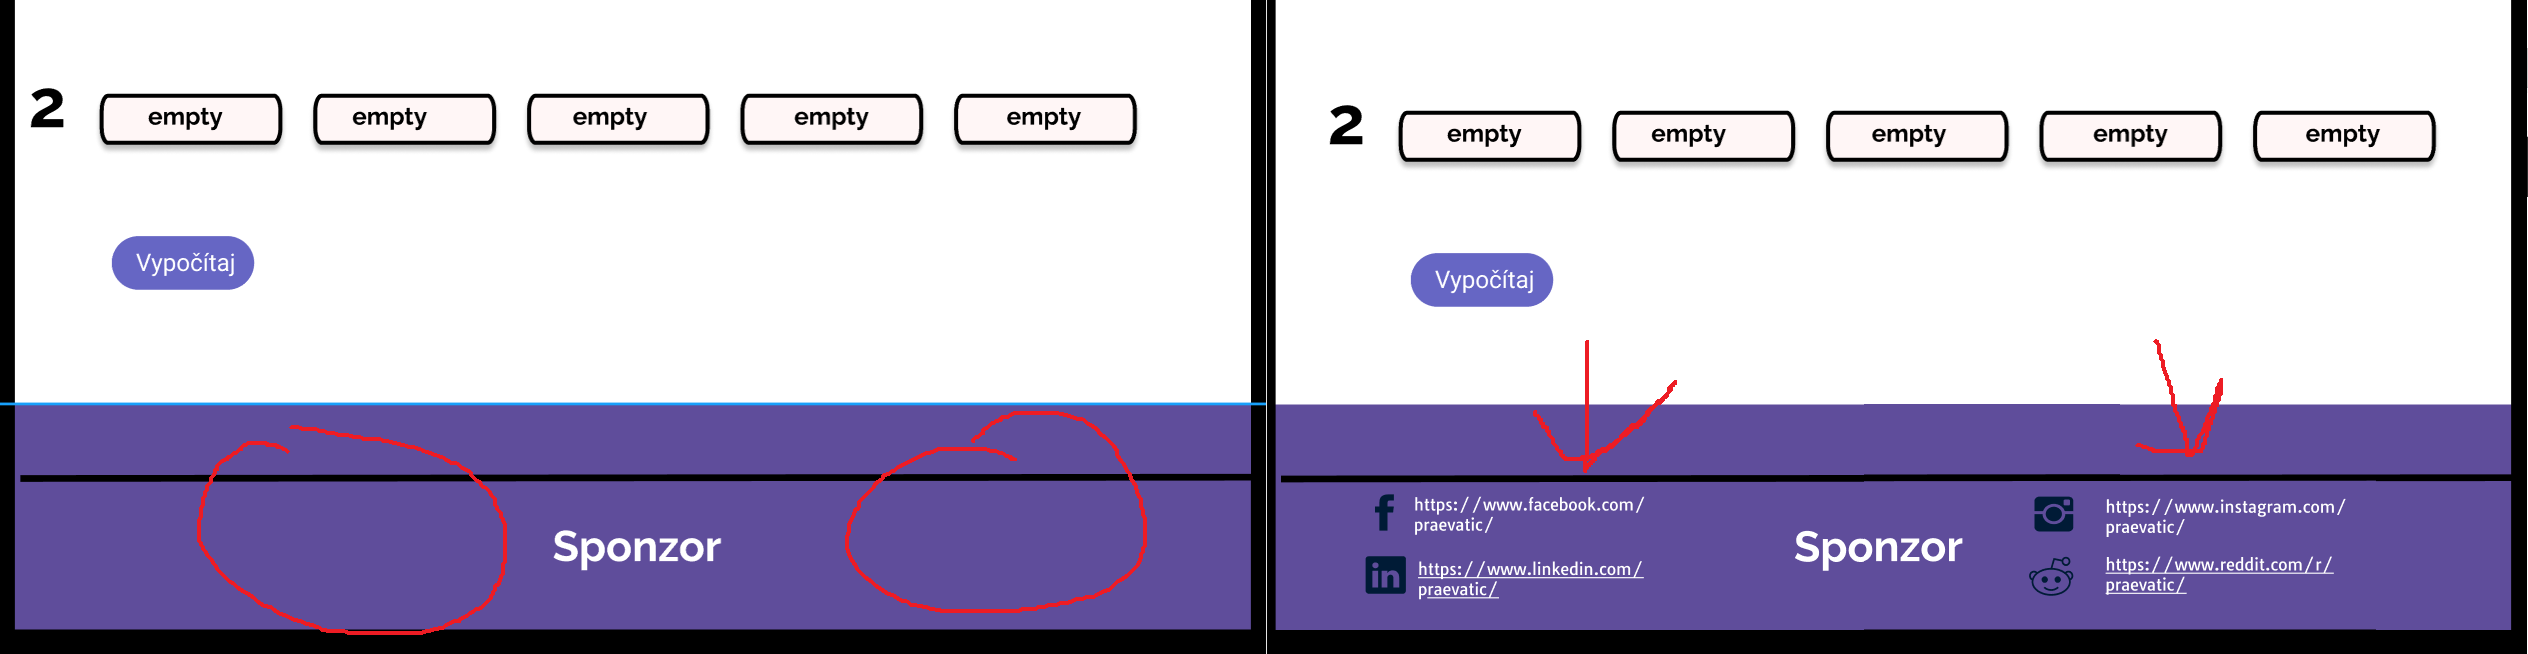
\includegraphics[width=.9\textwidth]{figures/4}
	
	\centering
	
	\caption{ Pridanie sociálnych sietí \label{4}}
	
\end{figure}

Kedže by bolo vhodné mať kontakt so zákazníkmi, aby mali možnosť sledovať zmeny alebo sa zapájať do debát s inými používateľmi, boli pridané sociálne siete\ref{4}, ktoré sú vhodným prostriedkom.





\section{Overenie prvého prototypu}



Účastníci hlavného testu boli 4 hráči, ktorí majú nahraté aj hry spomínané v tejto bakalárskej práci. Sú to 3 študenti, z toho 2 vysokoškoláci a 1 maturant a jeden pracujúci. Výsledky SUS dotazníka spomedzi účastníkov boli priemerne 95/100, čo je asi dôsledkom malého počtu účastníkov a zároveň aj vysokej jednoduchosti použitia. Aj keď výsledky SUS boli povzbudzujúce a utvrdili teóriu jednoduchosti používania, nevyšli z nich žiadne praktické výsledky. Na konkrétne podstatné zmeny bolo určené interview a zároveň pozorovanie účastníkov pri vykonávaní scenárov. Bolo potrebné urobiť viacero štylistických zmien na zlepšenie viditeľnosti niektorých popisov, ktoré pripomínali tlačidlá, takisto niektoré prechody a celkovú čitateľnosť. Vykonávanie scenárov a prvé dojmy účastníkov sú zaznamenané a uložené.


